%----------------------------------------------------------------------------------------
%	PACKAGES AND THEMES
%----------------------------------------------------------------------------------------
\documentclass[aspectratio=169,xcolor=dvipsnames]{beamer}
\usetheme{SimplePlus}

\usepackage[brazilian]{babel}
\usepackage[utf8]{inputenc}
\usepackage{hyperref}
\usepackage{graphicx} % Allows including images
\usepackage{booktabs} % Allows the use of \toprule, \midrule and \bottomrule in tables
% \usepackage[table,dvipsnames]{xcolor}
\usepackage{tikz,tkz-base, tkz-fct,tikz-3dplot,tikz-cd,tkz-tab,tkz-euclide,pgf,pgfplots}
\usepackage{pstricks}
\usepackage{pst-plot}
\usepackage{systeme}
\usepackage{multicol}
\usepackage{lmodern,mathrsfs}
\usepackage{tasks}
\usepackage{float}
\usepackage{array}
\usepackage{multirow}
\usetikzlibrary{matrix} % LATEX and plain TEX

\pgfplotsset{compat=newest}

%----------------------------------------------------------------------------------------
%	TITLE PAGE
%----------------------------------------------------------------------------------------

\title[short title]{Matrizes} % The short title appears at the bottom of every slide, the full title is only on the title page
% \subtitle{Subtitle}

\author[Fernando-Jorge] {Fernando Jorge}

\institute[NTU] % Your institution as it will appear on the bottom of every slide, may be shorthand to save space
{
  Escola Estadual Professor Lima Castro
}
\date{\today} % Date, can be changed to a custom date


%----------------------------------------------------------------------------------------
%	PRESENTATION SLIDES
%----------------------------------------------------------------------------------------

\begin{document}

\begin{frame}
    % Print the title page as the first slide
    \titlepage
\end{frame}

\begin{frame}{Sumário}
    % Throughout your presentation, if you choose to use \section{} and \subsection{} commands, these will automatically be printed on this slide as an overview of your presentation
    \tableofcontents
\end{frame}

%------------------------------------------------
\section{Introdução}
%------------------------------------------------

\begin{frame}{Definição}
  O que é uma Matriz?
  \begin{figure}[htb!]
    \centering
    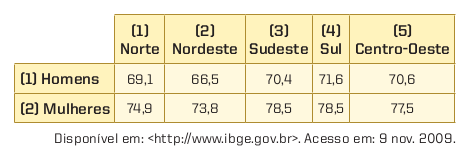
\includegraphics[width=.6\linewidth]{images/quadro.png}
  \end{figure}
  Matriz é toda tabela de números dispostos por linhas e colunas.

  Sabendo disso, qual a expectativa de vida de uma mulher residente na região Sul do país?
\end{frame}

%------------------------------------------------

\begin{frame}{Definição}
  Veja a tabela do slide anterior disposta como uma Matriz.
  \begin{center}
    \begin{tikzpicture}
      \matrix (magic) [matrix of nodes,ampersand replacement=\&, left delimiter=(, right delimiter=)]
      {
        69.1 \& 66.5 \& 70.4 \& 71.6 \& 70.6 \\
        74.9 \& 73.8 \& 78.5 \& |[red]| 78.5 \& 77.5 \\
      };
      \tkzDefPoint(2.6,-0.6){A}
      \tkzLabelPoint[right](A){\footnotesize$2 \times 5$}

      \draw[thick,red,->] (2.8,-0.8) to (2.8,-1.8);
      \tkzText[color=cyan](2.9,-2){Número de Linhas (m)}

      \draw[thick,red,->] (3.37, -0.4) |- (4.6,0);
      \tkzText[color=cyan](6.6,0){Número de Colunas (n)}

      \draw[thick,red,->] (magic-2-4) |- (0,-1.5);
      \tkzText[color=cyan, left](0,-1.48){Linha 2, Coluna 4}
    \end{tikzpicture}
  \end{center}
  Toda Matriz é representada por parênteses () ou colchetes [].

  A Matriz acima é do tipo $2 \times 5$, pois tem 2 linhas e 5 colunas.

\end{frame}

%------------------------------------------------

\begin{frame}{Representação Genérica}  
  Indicamos por \textbf{$a_{ij}$} o elemento posicionado na linha \textit{i} e na coluna \textit{j} de uma matriz \textit{A}.

  Na matriz:

  \begin{equation*}
    A_{3 \times 2} = \begin{bmatrix}
      6 & 7 \\
      -4 & 0 \\
      2 & -1
    \end{bmatrix}
  \end{equation*}

  \begin{itemize}
    \item o elemento 6 está na linha 1 e na coluna 1; por isso, ele é indicado por $a_{11}$, ou seja, $a_{11} = 6$;
    \item o elemento 7 está na linha 1 e na coluna 2; por isso, ele é indicado por $a_{12}$, ou seja, $a_{12} = 7$;
    \item analogamente, temos $a_{21} = -4$, $a_{22} = 0$, $a_{31} = 2$, $a_{32} = -1$.
  \end{itemize}
\end{frame}

%------------------------------------------------

\begin{frame}{Representação Genérica}
  Representamos genericamente uma matriz \textit{A} do tipo $m \times n$ da seguinte maneira:

  \begin{equation*}
    A_{m \times n} = \begin{bmatrix}
      a_{11} & a_{12} & a_{13} & \dots & a_{1n} \\
      a_{21} & a_{22} & a_{23} & \dots & a_{2n} \\
      \vdots & \vdots & \vdots & \vdots & \vdots \\
      a_{m1} & a_{m2} & a_{m3} & \dots & a_{mn} \\
    \end{bmatrix}
  \end{equation*}

  Forma abreviada: $A = (a_{ij})_{m \times n}$
  
\end{frame}

%------------------------------------------------

\begin{frame}{Representação Genérica}
  \begin{examples}
    Representar explicitamente a matriz $A = (a_{ij})_{2 \times 4}$ tal que $a_{ij} = 2i + j$.
  \end{examples}
\end{frame}

%------------------------------------------------

\begin{frame}{Matrizes Especiais}
  \begin{columns}[c] % The "c" option specifies centered vertical alignment while the "t" option is used for top vertical alignment

    \column{.5\textwidth} % Left column and width
      \begin{center}
        \begin{tikzpicture}
          \tkzText[color=brown, thick](0,1.5){Matriz Quadrada}
          \matrix (magic) [matrix of nodes,ampersand replacement=\&, left delimiter=(, right delimiter=)]
          {
            4 \& 9 \& 0 \\
            -6 \& 2 \& 4 \\
            3 \& 5 \& -2 \\
          };
        \end{tikzpicture}
      \end{center}
        \begin{center}
          Ordem da Matriz: 3
        \end{center} 

    \column{.5\textwidth} % Right column and width
      \begin{figure}[htb!]
        \centering
        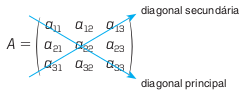
\includegraphics[width=1.0\linewidth]{images/quadrada.png}
      \end{figure}
      Obs: Apenas matrizes quadradas possuem diagonal principal e secundária.
      
      Diag. Princ: $i = j$

      Diag. Secun: $i + j = n + 1$

  \end{columns}
  
\end{frame}

%------------------------------------------------

\begin{frame}{Matrizes Especiais}
  \begin{multicols}{2}
    \centering Matriz Identidade ($I_n$)
    \vspace{.3cm}

    $I_3 = \begin{bmatrix}
      1 & 0 & 0 \\
      0 & 1 & 0 \\
      0 & 0 & 1
    \end{bmatrix}$
    \vspace{.3cm}

    $I_2 = \begin{bmatrix}
      1 & 0 \\
      0 & 1
    \end{bmatrix}$

  \centering Matriz Nula
    \vspace{.3cm}

    $\begin{bmatrix}
      0 & 0 & 0 \\
      0 & 0 & 0 \\
      0 & 0 & 0 \\
    \end{bmatrix}$
    \vspace{.3cm}

    $\begin{bmatrix}
      0 & 0 \\
      0 & 0 \\
    \end{bmatrix}$
    
  \end{multicols}
  
\end{frame}

%------------------------------------------------

\begin{frame}{Matrizes Especiais}
  Transposta de uma Matriz -- Troca-se linhas por colunas $M^t$
  \begin{tasks}
    \task {A transposta de $A_{3 \times 2} = \begin{bmatrix}
        5 & -4 \\
        6 & 2 \\
        0 & 7
    \end{bmatrix}$
    é a matriz $A^t_{2 \times 3} = \begin{bmatrix}
      5 & 6 & 0 \\
      -4 & 2 & 7 \\
    \end{bmatrix}$
    }

    \task {A transposta de $B_{1 \times 4} = \begin{bmatrix}
        2 & 0 & -5 & 8 \\
    \end{bmatrix}$
    é a matriz $B^t_{4 \times 1} = \begin{bmatrix}
      2 \\
      0 \\
      -5 \\
      8
    \end{bmatrix}$
  }
  \end{tasks}
  
\end{frame}

%------------------------------------------------

\begin{frame}{Matrizes Especiais}
  \begin{center}
    Igualdade de Matrizes
  \end{center}

  Duas Matrizes do mesmo tipo são iguais quando todos os elementos correspondentes são iguais.

  \begin{examples}
    Determinar o número real \textit{x} tal que: $\begin{bmatrix}
      6 & x^2-5 \\
      0 & x
    \end{bmatrix} = \begin{bmatrix}
      6 & 11 \\
      0 & 4
    \end{bmatrix}$
    
  \end{examples}
\end{frame}

%------------------------------------------------

\begin{frame}{Exercícios Propostos}
  \centering Resolver os exercícios do pdf de Matrizes: pg 4.
  
\end{frame}

%------------------------------------------------

%------------------------------------------------

\begin{frame}
    \Huge{\centerline{\textbf{Fim}}}
\end{frame}

%----------------------------------------------------------------------------------------

\end{document}
